\chapter{基于蒙特卡罗树搜索的模式文本匹配}
\label{chap:Zero}
利用 value iteation 可以解决大部分文本匹配的问题,但是 value iteration 基于贪心的路径搜索难以解决语言的组合结构问题。对于词序的微小变化导致的语义差别, value iteration 往往难以识别。而且 value iteration 在小数据集下容易陷入局部最优而导致算法严重过拟合。而 AlphaGo 以及 AlphaGo Zero 通过引入蒙特卡罗搜索树很好地解决了路径搜索中的贪心导致的局部最优解问题。本章介绍了蒙特卡罗树搜索相关算法并提出了基于蒙特卡罗树搜索的文本匹配算法。

\section{AlphaGo Zero 算法介绍}
\subsection{蒙特卡罗树搜索介绍}\label{sec:MCTS_intro}
蒙特卡罗树搜索\cite{Coulom2006EfficientSA} 在 2006 年被提出并在过去十多年中广泛用于各种游戏的人工智能\cite{Lorentz2008AmazonsDM, Enzenberger2010FuegoA,Buro2009ImprovingSE}。蒙特卡罗树搜索每次循环包含四步:

1. 选择(selecion):从根节点 R 开始,依次选择最佳的子节点,直到达到叶节点。选择最佳子节点的难点主要在于为了探索解空间需要维持较高的探索次数和利用现有模拟结果以加快训练速度。第一次解决探索和利用平衡的方法被称为上限置信区间算法\cite{Kocsis2006BanditBM}(Upper Confidence Bound 1 applied to trees),该方法基于 UCB1 \cite{Auer2002FinitetimeAO},建议在选择子节点时,以最大化 $\frac{w_i}{n_i} + c\sqrt{\frac{\ln N_i}{n_i}}$ 为目标。式中 $w_i$ 表示第 $i$ 次移动后的取胜次数;$n_i$ 表示第 $i$ 次移动后的仿真次数; $N_i$ 表示总仿真次数, $c$ 表示探索参数。

2. 扩展(expansion): 如果游戏没有结束,那么扩展叶节点,将一个或多个可用节点添加为该叶节点的子节点,并选择其中的一个子节点作为节点 C 。

3. 仿真(simulation): 从节点 C 开始,用随机策略选择节点进行游戏。

4. 反向传播(Backpropagation):根据仿真的结果更新从 C 到 R 的节点。

\begin{figure}[H]
    \centering
    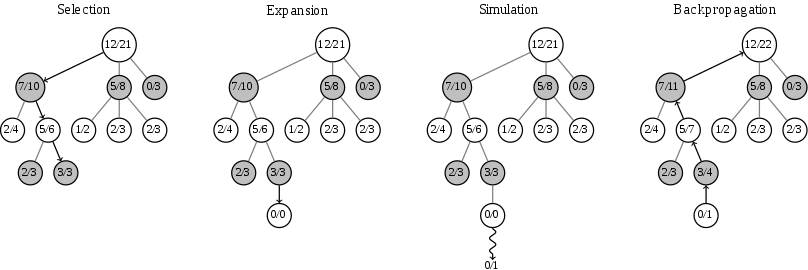
\includegraphics[width=1.0\textwidth]{MCTS}
    \bicaption{蒙特卡洛搜索树步骤}{Each Step of Monte Carlo tree search}
    \label{fig:MCTS}
\end{figure}

\subsection{AlphaGo}
\label{sec:AlphaGo}
AlphaGo 算法中存在 3 个网络:使用监督学习训练的策略网络 $p_\sigma$ 以及该网络的简化版 $p_\pi$;使用强化学习训练的策略网络 $p_\rho$ 以及价值网络 $v_\theta$。在树搜索的过程中,$p_\sigma$ 被用作模拟人类棋手落子;$p_\rho$ 决定落子位置,$v_\theta$ 判断当前局势。

$p_\sigma$ 的训练数据来自于 KGS 的三千万棋局,利用每个棋局及其对应的落子的数据,训练得到概率分布 $p_\sigma(a|s)$,即在当前状态(棋局)下采取行动(落子)的概率。由于 $p_\sigma$ 网络结构比较复杂,推导速度较慢,因此在 AlphaGo 算法训练时采用简化网络 $p_\pi$ 以降低训练速度;推导时采用 $p_\sigma$以提高胜率。

\begin{figure}[!htbp]
    \centering
    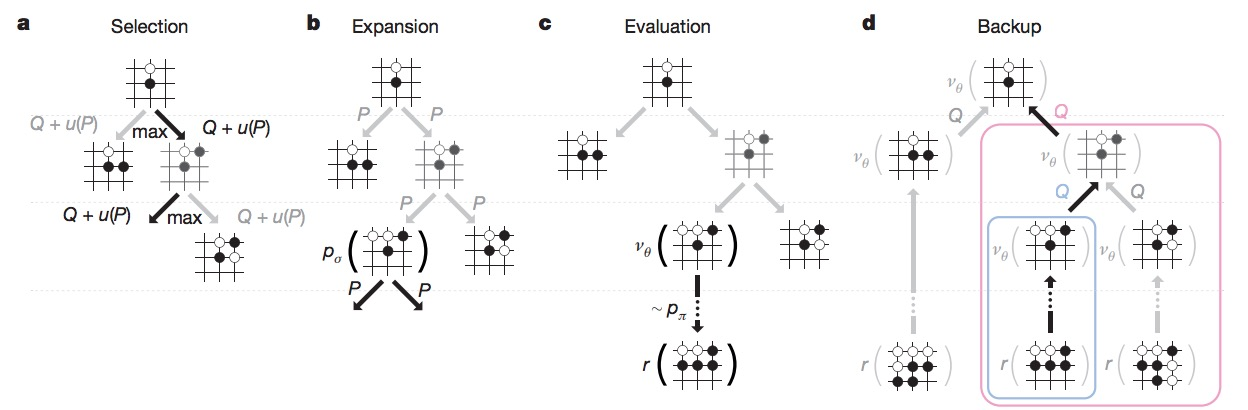
\includegraphics[width=1.0\textwidth]{Alpha_Go}
    \bicaption{AlphaGo 的树搜索过程}{Monte Carlo tree search in AlphaGo}
    \label{fig:Alpha_Go}
\end{figure}

蒙特卡罗树搜索使用随机进行仿真,Alpha Go 利用价值网络辅助策略网络作为落子参考进行仿真。图 \ref{fig:Alpha_Go} 中每一条边$(s, a)$ 都包含了行动价值$Q(s,a)$,该节点的访问次数$N(s,a)$以及先验概率$P(s,a) = p_\sigma(a|s)$。每次仿真从根节点开始根据当前状态 $s_t$ 选择行动 $a_t$ 直至到达叶节点。

\begin{equation}
\begin{aligned}
&a_t = \arg\max_a(Q(s_t,a) + u(s_t,a)) \\
&u(s_t,a) \propto \frac{P(s,a)}{1+N(s,a)}
\end{aligned}
\end{equation}

叶节点的重要程度由价值网络$v_\theta$ 和策略网络 $p_\pi$ 输出 $z_L$ 确定。

$$
V(s_L) = (1-\lambda)v_\theta(s_L) + \lambda z_L
$$

模拟结束时,所有边的行动价值以及参观次数都会被更新。
$$
\begin{aligned}
N(s,a) &= \sum_{i=1}^N\mathbf{1}(s,a,i)
Q(s,a) &= \frac{1}{N(s,a)}\sum_{i=1}^N\mathbf{1}(s,a,i)V(s_L^i)
\end{aligned}
$$

式中 $s_L^i$ 表示第 $i$ 次仿真的叶节点, $\mathbf{1}(s,a,i)$ 表示边 $(s,a)$ 是否被访问过。

\subsection{AlphaGo Zero}
AlphaGo Zero 是对 AlphaGo 的改进。相对于 AlphaGo,AlphaGo Zero 主要改进了以下几点:

1. AlphaGo Zero 是一个自训练的强化学习过程,不需要任何人类的先验知识;

2. AlphaGo Zero 仅仅使用围棋棋盘的黑白子作为输入,不需要其他人工抽取的特征;

3. AlphaGo Zero 将策略和价值网络融合,增强了网络的泛化能力;同时使用深度残差网络,网络深度加深,扩展了网络的解释能力;

AlphaGo Zero 使用了一个参数为 $\theta$ 的深度网络 $f_\theta$ ,该网络将棋盘作为输入,输出对应的概率和值函数 $(\mathbf{p}, v) = f_\theta(s)$. 式中 $\mathbf{p}$ 表示行动(落子)的概率$p_a = Pr(a|s)$, $v$ 是一个标量,表示当前棋局的胜率。

深度网络的训练仍然采用蒙特卡罗树搜索的方式。在时刻 $t$, 使用 $f_\theta$ 的输出为作参考进行下一轮蒙特卡罗树搜索,每一轮的树搜索都会输出当前状态(棋局)下每个行动(落子)的概率 $\mathbf{\pi}$。蒙特卡罗树搜索得到的落子概率比直接$f_\theta$  得到的落子概率更强,因此蒙特卡罗树搜索可以被认为是一个策略提升(policy improvement)的过程。利用$\mathbf{\pi}$进行落子后,不断循环直到棋局结束。在棋局结束后,将对弈者的胜负情况 $z$ 作为价值更新参数。最后更新$f_\theta$的网络参数以让 $f_\theta$ 的输出的落子概率和胜率 $(\mathbf{p}, v)$ 尽可能接近 $(\mathbf{\pi}, z)$,并在后面的棋局中使用新的参数来进行自对弈。

$f_\theta$ 的损失函数为:
$$
\ell = (z-v)^2 + \mathbf{\pi}^T\log \mathbf{p} + c\|\theta\|^2
$$
其中 $c$ 是正则化的系数。

蒙特卡罗树搜索以及参数更新的相关部分参考 \ref{sec:AlphaGo} 节。

\section{基于蒙特卡罗树搜索的文本匹配算法介绍}
在上一章,本文对文本匹配算法的 MDP 进行了介绍,本节对基于蒙特卡罗树搜索的文本匹配算法进行介绍。

\subsection{文本匹配 MDP 改进}
本节主要介绍对 \ref{sec:TM_MDP} 节所提到的 MDP 过程的改进。算法的整体流程和 \ref{sec:TM_MDP} 节相比没有太大改进,仍然是先生成匹配路径之后基于生成的路径判断是否匹配。

1. 状态 $\mathcal{S}$:我们将在 $t$ 时刻的状态 $s_t$ 定义为当前的路径以及从当前位置开始向前看的 $k$ 个单词:
$$
\begin{aligned}
\mathbf{Q}_t &= \{\mathbf{u}_{q_1}, \mathbf{u}_{q_2}, \mathbf{u}_{q_3}, \cdots, \mathbf{u}_{q_t}\},\\
\mathbf{D}_t &= \{\mathbf{v}_{d_1}, \mathbf{v}_{d_2}, \mathbf{v}_{d_3},\cdots, \mathbf{v}_{d_t}\},\\
\mathbf{F}_t &= \{[\mathbf{u}_{q_t}, \mathbf{v}_{d_t}], [\mathbf{u}_{1+q_t},\mathbf{v}_{1+d_t}] \cdots, [\mathbf{u}_{k+q_t}, \mathbf{v}_{k+d_t}]\},\\
s_t &= [\mathbf{Q}_t, \mathbf{D}_t, \mathbf{F}_t]
\end{aligned}
$$
式中 $q_t$ 和 $d_t$ 仍然表示当前位置, $\mathbf{Q}_t$ 和 $\mathbf{D}_t$ 表示输入的句子对 $Q, D$ 的前 $q_t$ 和 $d_t$ 按照路径拉伸得到的序列,$\mathbf{F}_t$ 表示从当前位置 $q_t, d_t$ 向前看 $k$ 个单词得到的序列。

2. 动作$\mathcal{A}$:在每个时间 $t$,我们都可以选择向下,向右或者像右下方行走。

3. 状态转移函数$\mathcal{T}(S,\mathcal{A})$:状态转移函数 $\mathcal{T}:S\times \mathcal{A}\rightarrow S$ 被定义为:
$$
(q_{t+1}, d_{t+1}) =
\begin{cases}
(q_{t} + 1, d_{t}) &\text{if goes down} \\
(q_{t}, d_{t} + 1) &\text{if goes right}  \\
(q_{t} + 1, d_{t} + 1) &\text{if goes obliquely}
\end{cases} \\
$$
$$
\begin{aligned}
s_{t+1} &= \mathcal{T}(s_t, a_t) = \mathcal{T}([\mathbf{Q}_t, \mathbf{D}_t, \mathbf{F}_t], a_t) = [\mathbf{Q}_{t+1}, \mathbf{D}_{t+1},\mathbf{F}_{t+1}]
\end{aligned}
$$
在每个时间 $t$:系统根据当前的状态选择一个行动(移动方向),并根据方向移动到下一个位置,状态随之转移:将当前位置两个句子的词向量分别添加到对应路径的末尾,更新未来单词序列。完成转移后,再根据当前状态继续移动。

4.值函数 $V$:值函数 $V: S\rightarrow \mathbb{R}$ 是对当前模型是否可以得到正确预测结果的预测。值函数需要不断更新以更加准确的得到预测结果。本节提出的值函数需要用到2个LSTM将 $Q_t$ 和 $D_t$ 映射为2个一维向量,并将结果定义为对这两个向量加权和的非线性转换:
\begin{equation}
\label{eq:MCTS_value}
V(s) = \sigma (<\mathbf{w}, \mathbf{g}_v(s)> + \mathbf{b}_v)
\end{equation}

式中 $\mathbf{w}, \mathbf{b}_v$ 是需要学习的参数,$
\sigma(x) = \frac{1}{1+e^{-x}}$ 是 sigmoid 函数以输出一个 0 $\sim$ 1 之间的概率,$\mathbf{g}_v(s)$ 是对将 LSTM$_Q$ 以及 LSTM$_D$ 的最后一层隐向量连接得到的:

\begin{equation}
\mathbf{g}_v(s) = [\mathrm{LSTM}_Q(\mathbf{Q}_t)^T, \mathrm{LSTM}_D(\mathbf{D}_{t})^T]^T
\end{equation}

LSTM 网络的定义和公式~\ref{eq:LSTM} 一致,LSTM$_Q$ 和 LSTM$_D$ 共享参数。

5. 策略函数 $\mathbf{\pi}$:$\mathbf{\pi}(s)$ 将环境状态作为输入,输出每个行动的概率。策略函数将 $\mathbf{g}_v(s), F_t$ 作为输入,使用一个 LSTM 将 $F_t$ 映射为一个一维向量,并将其和 $\mathbf{g}_v(s)$ 连接,将连接后的向量利用 softmax 函数进行归一化得到每个行动的概率分布:
\begin{equation}
\label{eq:MCTS_policy}
\begin{aligned}
\pi(a|s) &= \frac{\exp\left\{\Phi(a)^T \mathbf{U}_\pi ~\mathbf{g}_\pi(s)\right\}}{\sum_{a'\in\mathcal{A}(s)} \exp\left\{\Phi(a')^T \mathbf{U}_\pi ~\mathbf{g}_\pi(s)\right\}} \\
\mathbf{g}_\pi(s) &= [\mathbf{g}_v(s) , \mathrm{LSTM}_F(\mathbf{F}_{t})^T]^T
\end{aligned}
\end{equation}

\subsection{路径判别}
在 \ref{sec:path_classify} 中,我们提出了一种针对于路径的判别模型判断路径是否匹配。但是由于该方法在每次运行时的计算图都不尽相同,因此效率很低。本节对该方法进行了改进以提高其训练和推断速度。

判别模型将 $\mathbf{Q}_t$ 和 $\mathbf{D}_t$ 作为输入,并使用两个 LSTM 将其映射为2个矩阵,最后使用一个 LSTM 接受两个矩阵作为输入,输出一个一维向量:
$$
\begin{aligned}
\mathbf{g}_q &= \mathrm{LSTM}_Q(Q_t)\\
\mathbf{g}_d &= \mathrm{LSTM}_D(D_t)\\
\mathbf{g}_c^{\text{in}} &= [[\mathbf{g}_{q, 1}, \mathbf{g}_{d, 1}], [\mathbf{g}_{q, 2}, \mathbf{g}_{d, 2}], \cdots, [\mathbf{g}_{q, t}, \mathbf{g}_{d, t}]]\\
\mathbf{g}_c^{\text{out}} &= \mathrm{LSTM}_C({g}_c^{\text{in}})
\end{aligned}
$$
LSTM$_Q$和LSTM$_D$ 共享参数。最后输出概率会通过 sigmoid 函数变换概率输出:
\begin{equation}
\label{eq:classification_model}
p_m = \frac{1}{1+e^{-{\mathbf{g}_c^{\text{out}}}}}
\end{equation}

\begin{figure}[!htbp]
    \centering
    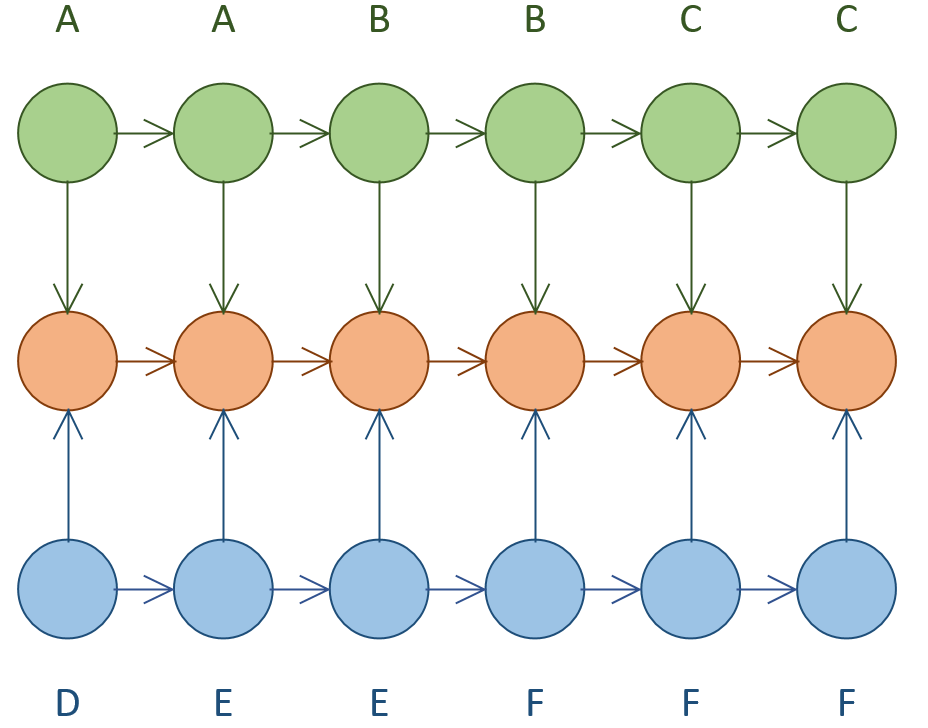
\includegraphics[width=0.4\textwidth]{MCTS_path}
    \bicaption{路径判别函数}{Path classifiction}
    \label{fig:MCTS_path}
\end{figure}

\subsection{蒙特卡罗树搜索的训练和推断}
\label{sec:MCTS_train}
在\ref{sec:lab_value} 节,本文通过在大数据和小数据集上的训练结果发现单纯将策略函数的输出作为行动概率很容易陷入局部最优解,即使使用 $\epsilon$-贪心的方式也很难摆脱。受 AlphaGo 和 AlphaGo Zero 的启发,本节使用蒙特卡罗树搜索的方式进行前向式搜索。在 $t$ 时刻,算法在策略和价值网络的辅助下执行一次蒙特卡罗树搜索,得到搜索策略 $\mathbb{\pi}$,并根据 $\pi$ 确定下一个行动的位置。

\begin{algorithm}[!htbp]
\caption{TreeSearch}\label{alg:TreeSearch}
\renewcommand{\algorithmicrequire}{\textbf{Input:}}
\renewcommand{\algorithmicensure}{\textbf{Output:}}
\begin{algorithmic}[1]
\Require root $s_R$, value $V$, policy $\pi$, search times $K$
\Ensure Search policy $\mathbf{\pi}$
\For{$k = 0$~$\text{to}$~$K-1$}
\State $s_L\leftarrow s_R$
\State {\{Selection\}}
\While{$s_L \textrm{ is not a leaf node}$}
  \State $a \leftarrow \arg\max_{a\in\mathcal{A}(s_L)} Q(s_L, a) +\lambda \cdot U(s_L, a)$\Comment{Eq.~(\ref{eq:Selection})}
  \State $s_L \leftarrow \textrm{ child node pointed by edge }(s_L, a)$
\EndWhile

\State {\{Evaluation and expansion\}}
%\IF{$s_L$ can be expanded}
    \State $v\leftarrow V(s_L)$ \Comment{simulate $v$ with value function $V$}
  \For{$\text{all }a \in\mathcal{A}(s_L)$}
    \State Expand an edge $e$ to node $ s = [s_L.\mathbf{Q}_t, s_L.\mathbf{D}_t, s_L.\mathbf{F}_t]$
    \State $e.P \leftarrow p(a|s_L); e.Q \leftarrow 0; e.N \leftarrow  0$\Comment{init edge properties}
  \EndFor
%\ELSE
% \State{$v\leftarrow\left\{\begin{array}{cl} V(s_L) & R= NULL\textrm{ or }J=\emptyset \\ R(s_L.\mathcal{Z}, J) & \textrm{others}\\ \end{array} \right.$}\Comment{simulate with $V$ at test phase ($R=NULL$ or $J=\emptyset$), or directly set to its real value (e.g., $\alpha$-NDCG) at the training phase}
%\ENDIF
\State {\{Back-propagation\}}
\While{$s_L \neq s_R$}
  \State $s \leftarrow \textrm{ parent of }s_L; e \leftarrow \textrm{ edge from }s\textrm{ to }s_L$
  \State $e.Q \leftarrow \frac{e.Q\times e.N + v}{e.N + 1}$\Comment{Equation~(\ref{eq:UpdateQN})}
  \State $e.N \leftarrow e.N + 1; s_L \leftarrow s$
\EndWhile
\EndFor

\State {\{Calculate tree search policy. Eq.~(\ref{eq:SearchProb})\}}
\For{$\text{all }a\in\mathcal{A}(s_R)$}
  \State $\pi(a|s_R)\leftarrow \frac{e(s_R, a).N}{\sum_{a'\in\mathcal{A}(s_R)}e(s_R, a').N}$
\EndFor
\Return $\mathbf{\pi}$
\end{algorithmic}
\end{algorithm}

Alg~\ref{alg:TreeSearch} 展示了蒙特卡罗树搜索的细节,其中每一个树节点对应一个状态。算法以根节点 $s_R$、值函数 $\mathcal{V}$ 以及策略函数 $\pi$ 作为输入,输出策略 $\mathbb{\pi}$。算法会迭代 $K$ 次,每次从 $s_P$ 开始选择一个方向移动。搜索树中每条边$e(s,a)$都存储着行动价值 $Q(s,a)$ 参观次数 $N(s,a)$ 以及先验概率 $\pi(s,a)$。每次迭代式,会执行以下操作:

1. 选择:每次迭代都从根节点 $s_R$ 开始,以最大化上限置信区间为目标选择行动:
\begin{equation}\label{eq:Selection}
  a_t = \arg\max_a (Q(s_t, a) + \lambda U(s_t, a)),
\end{equation}
式中 $\lambda >0$ 是权衡系数,$U(s_t, a) =  p(a|s_t)\frac{\sqrt[]{\sum_{a'\in\mathcal{A}(s_t)} N(s_t, a')}}{1 + N(s_t, a)}$. $U(s_t, a)$ 和先验概率有关但是随着参观次数的增加而逐渐减小。

2. 评价扩展:到达叶节点时,节点会根据值函数 $V(s_L)$ (公式~\ref{eq:MCTS_value}) 计算当前节点的价值。如果搜索过程没有结束,则该节点需要被扩展。新的叶节点状态 $s_L$ 会被初始化为 $\pi(s_L, a) =\pi(a|s_L)$ (公式~\ref{eq:MCTS_policy}), $Q(s_L, a)= 0$, $N(s_L, a) = 0$。本节介绍的算法会始终扩展叶节点直到到达矩阵右下角。

3. 回溯更新:评价结束时,每条边都会被更新:
\begin{equation}
\label{eq:UpdateQN}
\begin{aligned}
  &Q(s, a) \leftarrow  \frac{Q(s, a) \times N(s, a) + V(s_L)}{N(s, a) + 1}\\
  &N(s, a) \leftarrow  N(s, a) + 1.
\end{aligned}
\end{equation}

4. 计算策略:在 $K$ 次迭代结束后,根据根节点 $s_L$ 每条边的访问次数确定每个行动的概率:
\begin{equation}\label{eq:SearchProb}
\pi(a|s_R) = \frac{N(s_R, a)^{\frac{1}{\tau}}}{\sum_{a'\in\mathcal{A}(s_R)} N(s_R, a')^{\frac{1}{\tau}}},
\end{equation}
式中 $\tau > 0$ 表示系统温度。

\subsubsection{模型的训练}
本章提出的模型的参数 $\Theta_{MCTS}$(包含 $\mathbf{w}, b_v, \mathbf{U}_p$, 以及 LSTM$_D$, LSTM$_Q$ 和 LSTM$_F$中的参数),$\Theta_{c}$(包含LSTM$_D$, LSTM$_Q$ 和 LSTM$_c$ 中的参数)需要在训练时被更新。在训练阶段,算法接受 $N$ 个标记的句子对 $D = \{ (\mathbf{Q}^{(n)}, \mathbf{D}^{(n)}), \mathbf{Y}\}_{n=1}^{N}$。算法~\ref{alg:Train}展示了整个训练过程。首先将参数  $\Theta_{MCTS}$ 和 $\Theta_{c}$ 初始化为 $[-1, 1]$ 的随机数,每轮迭代时,对于每个句子对 $(\mathbf{Q}, \mathbf{D})$,我们都需要预测一条路径。在每个时间 $t$都会执行一次蒙特卡洛树搜索,并输出策略 $\mathbb{\pi}$,根据策略随机采样出对应的移动方向 $a_t$,直到到达匹配矩阵的右下角。在得到一条路径 $([u_{q_1}, u_{q_2}, \cdots, u_{q_t}], [v_{d_1}, v_{d_2}, \cdots, v_{d_t}])$ 后,使用交叉熵损失更新路径判别模型:

\begin{equation}
\label{eq:classification_loss}
\ell_c(Y, p) = -\left(Y\log(p) + (1-Y)\log (1-p)\right)
\end{equation}

在路径判别模型收敛后,对每条路径进行预测得到标签 $Y_p$,并根据 $Y_p$ 与实际标签 $Y$ 计算奖励 $r= \mathbb{I}_{\mathbf{Y} = \mathbf{Y}_p}$。蒙特卡罗树搜索中每一轮生成的数据 $E=\{s_t, \mathbb{\pi}_t\}$ 以及 $r$ 会被用作更新价值和策略网络,使其输出的值 $V(s_t)$和策略$\mathbb{p}(s_t)$ 尽可能逼近 $r$ 和 $\mathbb{p}(s_t)$。该网络的损失函数为:
\begin{equation}
\label{eq:loss}
\begin{aligned}
  \ell(E, r) = &\sum_{t=1}^{|E|} (-(r\log V(s_t) + (1-r)\log (1-V(s_t)))  \\
  &+ \beta\sum_{a\in\mathcal{A}(s_t)}\pi_t(a|s_t) \log \frac{1}{\pi(a|s_t)}).
\end{aligned}
\end{equation}
模型通过反向传播和离散梯度下降更新。

\begin{algorithm}[!htbp]
\caption{Train text matching model}\label{alg:Train}
\renewcommand{\algorithmicrequire}{\textbf{Input:}}
\renewcommand{\algorithmicensure}{\textbf{Output:}}
\begin{algorithmic}[1]
\Require Labeled data $D=\{ (\mathbf{D}^{(n)}, \mathbf{Q}^{(n)}, \mathbf{Y}^{(n)})\}_{n=1}^N$, learning rate $\eta$, number of search $K$
\Ensure $\Theta_{MCTS}, \Theta_{c}$
\State \text{Initialize} $\Theta_{MCTS}, \Theta_{c} \leftarrow$ random values in $[-1, 1]$
\Repeat
  \For{$(\text{all }\mathbf{X}, \mathbf{Y})\in D$}
    \State {$s \leftarrow [\{\mathbf{u}_1\}, \{\mathbf{v}_1\}, \{[\mathbf{u}_1,\mathbf{v}_1], \cdots, [\mathbf{u}_k, \mathbf{v}_k]\}]$}
    \While{not reach right down corner}
            \State $\mathbb{\pi} \leftarrow \mathrm{TreeSearch}(s, V, \mathbf{p}, K)$ \Comment{Alg.~(\ref{alg:TreeSearch})}
      \State sample action ${a\in\mathcal{A}(s)}$ according to $\pi(a|s)$
      \State $E\leftarrow E \oplus \{(s, \mathbb{\pi})\}$
      %\State $[\mathbf{q}, \mathcal{Z}, X]\leftarrow s$
      \State $s \leftarrow [s.\mathbf{Q}_{t+1}, s.\mathbf{D}_{t+1}, s.\mathbf{F}_{t+1}]$
    \EndWhile
    \While{\text{not convergence}}
    \State $\Theta_{c} \leftarrow \Theta_{c} - \eta \frac{\partial \ell_c(\mathbf{Y}, p)}{\partial \Theta_{c}}$  \Comment{$\ell_c$ is defined in Eq.~(\ref{eq:classification_loss})}
    \EndWhile
    \State compute $\mathbf{Y}_p$ by Eq.~(\ref{eq:classification_model})
    \State $r \leftarrow \mathbb{I}_{\mathbf{Y} = \mathbf{Y}_p}$
    \State $\Theta_{MCTS} \leftarrow \Theta_{MCTS} -\eta \frac{\partial \ell(E, r)}{\partial \Theta_{MCTS}}$ \Comment{$\ell$ is defined in Eq.~(\ref{eq:loss})}
  \EndFor
\Until {converge}
\State\Return $\Theta_{MCTS}, \Theta_{c}$
\end{algorithmic}
\end{algorithm}

\subsubsection{模型的推断}
算法~\ref{alg:Train}展示了模型的推断过程。给定一个句子对 $\mathbf{Q}, \mathbf{D}$,系统的初始化状态 $s_1=[\{\mathbf{u}_1\}, \{\mathbf{v}_1\}, \{[\mathbf{u}_1,\mathbf{v}_1], \cdots, [\mathbf{u}_k, \mathbf{v}_k]$。在每个时间节点 $t$,主体都会得到系统的状态 $s_t=[\mathbf{Q}_t, \mathbf{D}_t, \mathbf{F}_t]$ 以及蒙特卡罗树搜索得到的策略 $\mathbb{\pi}$,根据 $\mathbb{\pi}$ 做出行动后更新当前状态得到 $s_{t+1}$。该过程不断持续直到到达匹配矩阵的右下角。

\begin{algorithm}[!htbp]
\caption{Text matching Inference}\label{alg:RLRank_MCTS}
\renewcommand{\algorithmicrequire}{\textbf{Input:}}
\renewcommand{\algorithmicensure}{\textbf{Output:}}
\begin{algorithmic}[1]
\Require sentence pair $\mathbf{Q}=\{\mathbf{u}_1, \cdots, \mathbf{u}_M\}$, $\mathbf{D}=\{\mathbf{w}_1, \cdots, \mathbf{w}_M\}$, value function $V$, policy function $\mathbf{p}$, and search times $K$,
\Ensure label $\mathbf{Y}$
\State $s \leftarrow [\{\mathbf{u}_1\}, \{\mathbf{v}_1\}, \{[\mathbf{u}_1,\mathbf{v}_1], \cdots, [\mathbf{u}_k, \mathbf{v}_k]\}]$
\While{not reach right down corner}
  \State $\mathbb{\pi} \leftarrow \mathrm{TreeSearch}(s, V, \mathbf{p}, K)$
  \State $a \leftarrow \arg\max_{a\in\mathcal{A}(s)} \pi(a|s)$
% \State $[\mathbf{X}, \mathbf{Y}]\leftarrow s$
  \State $s \leftarrow [s.\mathbf{Q}_{t+1}, s.\mathbf{D}_{t+1}, s.\mathbf{F}_{t+1}]$
\EndWhile
\State compute $\mathbf{Y}_p$ by Eq.~(\ref{eq:classification_model})
\State \Return $\mathbf{Y_p}$
\end{algorithmic}
\end{algorithm}


\section{实验分析}
为了对我们提出的基于蒙特卡罗树搜索的文本匹配算法有效性进行评估,我们利用 Quora 的问题匹配数据集进行了测试。

\section{本章小结}
本章主要介绍了基于蒙特卡罗树搜索的文本匹配算法。首先我们对上一章提出的 MDP 进行了改进,加入了路径信息。路径信息的引入使得价值网络的预测更加精确。

为了解决直接使用价值网络输出的值函数会导致算法陷入局部最优解的问题,本章引入了蒙特卡罗树搜索算法,通过蒙特卡罗树搜索算法增强搜索策略的可用性,也解决了文本匹配中由于语言组合结构带来的语义区分问题。

最后本文在quora数据集上进行了测试,实验结果表明本文提出的模型具有优异的性能。
